\documentclass{article}
\usepackage{amsmath}
\usepackage{amssymb}
\usepackage{fullpage}
\usepackage[parfill]{parskip}
\usepackage{graphicx}
\newcommand*{\horzbar}{\rule[.5ex]{2.5ex}{0.5pt}}
\newcommand{\pd}[2]{\frac{\partial #1}{\partial #2}}
\title{Assignment 1 writeup}
\author{Thomas Lu}
\date{}
\begin{document}
\maketitle
\section{Problem 1}
(a) We have
\begin{align*}
\text{softmax}(\mathbf{x} + c)_i &= \frac{e^{x_i + c}}{\sum_j e^{x_j + c}}\\
&= \frac{e^c(e^{x_i})}{e^c\sum_j e^{x_j}}\\
&= \frac{e^c}{e^c} \frac{e^{x_i}}{\sum_j e^{x_j}}\\
&= \frac{e^{x_i}}{\sum_je^{x_j}}\\
&= \text{softmax}(\mathbf{x})_i,
\end{align*}
so $\text{softmax}(\mathbf{x} + c) = \text{softmax}(\mathbf{x}),$ as desired.

\section{Problem 2}
(a) We have
\begin{align*}
\sigma(x) &= \frac{1}{1 + e^{-x}}\\
\sigma'(x) &= \frac{d}{dx} (1 + e^{-x})^{-1}\\
&=  -(1 + e^{-x})^{-2}\frac{d}{dx}\left(1 + e^{-x}\right) \\
&= -\left(\frac{1}{1 + e^{-x}}\right)^2 \left(-e^{-x}\right)\\
&= \left(\frac{1}{1 + e^{-x}}\right)\left(1 - \frac{1}{1 + e^{-x}}\right)\\
&= \left(\sigma(x)\right)\left(1 - \sigma(x)\right).
\end{align*}

(b) We have $\hat{y} = \text{softmax}(\theta).$ Suppose that $y$ is one-hot with $y_k = 1$. Then
\begin{align*}
\frac{\partial}{\partial \theta_j} CE(y, \hat{y}) &= \frac{\partial}{\partial \theta_j} \sum_i -y_i \log \frac{e^{\theta_i}}{\sum_i e^{\theta_i}}\\
&= -\frac{\partial}{\partial \theta_j} \log\frac{e^{\theta_k}}{\sum_i e^{\theta_i}}\\
&= \frac{\partial}{\partial \theta_j} \left(\log\left(\sum_i e^{\theta_i}\right) - \log e^{\theta_k} \right)\\.
\end{align*}
We now split into two cases. If $j \ne k$, then
\begin{align*}
\frac{\partial}{\partial \theta_j} CE(y, \hat{y}) &= \frac{\partial}{\partial \theta_j} \left(\log\left(\sum_i e^{\theta_i}\right) - \log e^{\theta_k} \right)\\
&= \frac{1}{\sum_i e^{\theta_i}}(e^{\theta_j})\\
&= \text{softmax}(\theta)_j.
\end{align*}
If $j = k$, then
\begin{align*}
\frac{\partial}{\partial \theta_j} CE(y, \hat{y}) &= \frac{\partial}{\partial \theta_k} \left(\log\left(\sum_i e^{\theta_i}\right) - \log e^{\theta_k} \right)\\
&= \frac{1}{\sum_i e^{\theta_i}}(e^{\theta_k}) - \frac{\partial}{\partial \theta_k}\theta_k\\
&= \text{softmax}(\theta)_k - 1.
\end{align*}
Thus
$$\vec{\nabla}_{\theta} CE(y, \hat{y}) = \text{softmax}(\theta) - y.$$

(c) We begin with a couple of theorems:

\textbf{Theorem:} If $f_1, f_2, \dots, f_n, g$ are differentiable, and
$$y = g(f_1(x), f_2(x), \dots, f_n(x)),$$
then
$$\frac{dy}{dx} = \sum_{i=1}^n \frac{\partial y}{\partial f_i} \frac{df_i}{dx}.$$

\textbf{Theorem:} If $x$ and $y$ are row vectors and $z$ is a scalar, and $f$ and $g$ are differentiable with $y = f(x)$ and $z = g(y)$, then
$$\frac{\partial z}{\partial x} = \frac{\partial z}{\partial y}\frac{\partial y}{\partial x},$$
where
$$\left(\frac{\partial y}{\partial x}\right)_{ij} = \frac{\partial y_i}{\partial x_j}.$$

We now compute $\partial J/\partial x$. Letting $z_1 = xW_1 + b_1$ and $z_2 = hW_2 + b_2$, we have
$$\frac{\partial J}{\partial x} = \frac{\partial J}{\partial z_2} \frac{\partial z_2}{\partial h} \frac{\partial h}{\partial z_1} \frac{\partial z_1}{\partial x}.$$
We evaluate the partials on the RHS of the above equation in sequence. We have:
\begin{align*}
\frac{\partial J}{\partial z_2} &= \text{softmax}(z_2) - y\\
\frac{\partial z_2}{\partial h} &= W_2^T\\
\frac{\partial h}{\partial z_1} &= \text{diag}(\sigma(z_1))\text{diag}(1 - \sigma(z_1))\\
\frac{\partial z_1}{\partial x} &= W_1^T\\
\Rightarrow \frac{\partial J}{\partial x} &= (\text{softmax}(z_2) - y)W_2^T\text{diag}(\sigma(z_1))\text{diag}(1 - \sigma(z_1))W_1^T\\
&= (\text{softmax}(z_2) - y) W_2^TW_1^T\circ \sigma(z_1) \circ (1 - \sigma(z_1))
\end{align*}
where $\text{diag}(v)$ denotes the diagonal matrix $D$ with $D_ii = v_i$ and 1 denotes a vector of ones where appropriate.

(d) There are four groups of parameters:
\begin{itemize}
\item $b_1$, a bias vector with $H$ entries,
\item $b_2$, a bias vector with $D_y$ entries,
\item $W_1$, a $D_x \times H$ weight matrix, and
\item $W_2$, a $H \times D_y$ weight matrix.
\end{itemize}
Thus the total number of parameters is
$$H + D_y + HD_x + HD_y = D_y(H + 1) + H(D_x + 1).$$

\section{Problem 3}
(a) Let $V$ be our vocabulary, and for $o, c \in V$, let $v_c$ denote the center word (column) vector for $c$ and $u_o$ denote the outer word (column) vector for $o$. Let $U$ denote the matrix
$$
\left[
\begin{array}{ccc}
\horzbar & u_{w_1}^T \horzbar \\
\horzbar & u_{w_2}^T \horzbar \\
& \vdots & \\
\horzbar & u_{w_N}^T \horzbar \\
\end{array}
\right],
$$
where $V = \{w_1, w_2, \dots, w_N\}$. Let 
$$\hat{y}_i = p(w_i | c) = \frac{\exp(u_{w_i}^Tv_c)}{\sum_{w \in V}\exp(u_w^Tv_c)}$$
and $\hat{y} = [\hat{y}_1, \hat{y}_2, \dots, \hat{y}_N].$ Supposing that $y$ is one-hot with the one at $o$, we have
\begin{align*}
\pd{J}{v_c} &= \pd{}{v_c} CE(y, \hat{y})\\
&= -\pd{}{v_c} \sum_{i=1}^N y_i \log \hat{y}_i \\
&= -\pd{}{v_c} \log \frac{\exp(u_o^Tv_c)}{\sum_{w\in V} \exp\left(u_w^Tv_c\right)}\\
&= -\pd{}{v_c} \left( \log\left(\exp(u_o^Tv_c)\right) - \log\left(\sum_{w\in V} \exp\left(u_w^Tv_c\right)\right)\right)\\
&= -u_o + \frac{1}{\sum_{w\in V}\exp( u_w^Tv_c)} \sum_{w\in V}\pd{}{v_c}\exp\left(u_w^Tv_c\right)\\
&= -u_o + \frac{1}{\sum_{w\in V}\exp( u_w^Tv_c)} \sum_{w\in V}u_w\exp\left(u_w^Tv_c\right)\\
&= -u_o + \sum_{i=1}^N u_{w_i}\hat{y}_i\\
&= U^T\left(\hat{y} - y\right).
\end{align*}

(b) We have, using the same variable conventions as in (a),
\begin{align*}
\pd{J}{u_{w_i}} &= -\pd{}{u_{w_i}} \log \frac{\exp(u_o^Tv_c)}{\sum_{w\in V} \exp\left(u_w^Tv_c\right)}\\
&= -\pd{}{u_{w_i}} \left( \log\left(\exp(u_o^Tv_c)\right) - \log\left(\sum_{w\in V} \exp\left(u_w^Tv_c\right)\right)\right)\\
&= -v_c(1_{w_i = o}) + \frac{1}{\sum_{w\in V}\exp( u_w^Tv_c)} \pd{}{u_{w_i}} \left(\sum_{w \in V}\exp\left(u_w^Tv_c\right) \right)\\
&= -v_c(1_{w_i = o}) + \left(\frac{\exp\left(u_{w_i}^Tv_c\right)}{\sum_{w\in V}\exp( u_w^Tv_c)} \right)v_c\\
&= -v_cy_i + \hat{y}_i v_c\\
\Rightarrow \pd{J}{U} &= (\hat{y} - y)v_c^T.
\end{align*}

(c) Note first that
$$\frac{d}{dx} \log(\sigma(x)) = \frac{1}{\sigma(x)}\sigma'(x) = \frac{1}{\sigma(x)}\left(\sigma(x)(1 - \sigma(x))\right) = 1 - \sigma(x).$$
For $w \notin \{o, 1, 2, \dots, K\},$ it is clear that $\partial J/\partial u_w = 0$. Now
$$\pd{J}{u_o} = -(1 - \sigma(u_o^Tv_c))\pd{}{u_o}\left(u_o^Tv_c\right) = v_c(\sigma(u_o^Tv_c) - 1)$$
$$\pd{J}{u_i} = -\pd{}{u_i} \log\sigma(-u_i^Tv_c) = v_c(1 - \sigma(-u_i^Tv_c)),$$
where $i \in \{1, 2, \dots, K\}.$ Similarly, we can compute
$$\pd{J}{v_c} = u_o(\sigma(u_o^Tv_c) - 1) + \sum_{k=1}^K u_k(1 - \sigma(-u_k^Tv_c)).$$
This is much faster to compute because we only need to perform $K/V$ (proportionally) as many dot products.

(d) For the skip-gram model, we have
\begin{align*}
\pd{J_{\text{skipgram}}(w_{t-m \dots t+m})}{v_c} &= \sum_{\substack{t-m \le j \le t+m\\j \ne 0}} \pd{F(w_j, v_c)}{v_c}\\
\pd{J_{\text{skipgram}}(w_{t-m \dots t+m})}{v_j} &= 0, ~ j\ne c\\
\pd{J_{\text{skipgram}}(w_{t-m \dots t+m})}{U} &= \sum_{\substack{t-m \le j \le t+m\\j \ne 0}} \pd{F(w_j, v_c)}{U}\\
\end{align*}
For CBOW, we have
\begin{align*}
\pd{J_{\text{CBOW}}(w_{t-m \dots t+m})}{v_c} &= \pd{F(w_t, \hat{v})}{\hat{v}} \pd{\hat{v}}{v_c} = \pd{F(w_t, \hat{v})}{\hat{v}}\\
\pd{J_{\text{CBOW}}(w_{t-m \dots t+m})}{U} &= \pd{F(w_t, \hat{v})}{U}\\
\pd{J_{\text{CBOW}}(w_{t-m \dots t+m})}{v_j} &= 0, ~ j \ne c.
\end{align*}

(g)

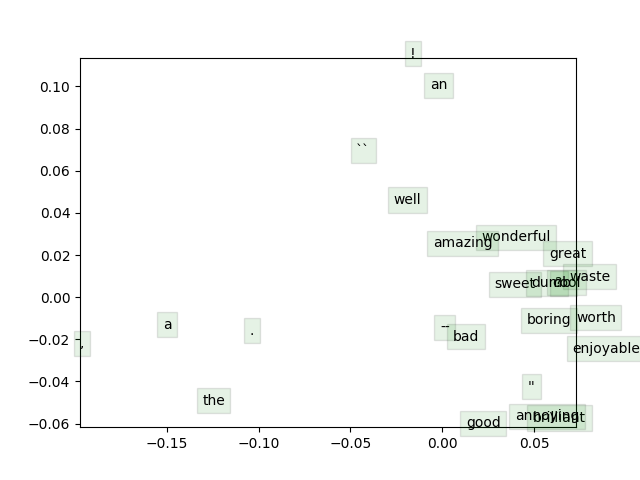
\includegraphics{assignment1/q3_word_vectors.png}

The plot is a 2-D projection of the word vectors trained from our corpus. We see that a number of generic quality-describing adjectives are clustered together (amazing, wonderful, great) along with some less general but still quite versatile ones (sweet, dumb, boring, enjoyable). Interestingly, ``waste" is also clustered pretty closely to these words; it is often used in a similar context (``x was a waste of time" vs. ``x was boring") although it is a noun rather than an adjective.

\section{Problem 4}
(b) Regularization prevents overfitting by establishing a prior that all parameters of the model are close to zero. This incentivizes the model to only focus on the most informative features instead of overfitting on all the data provided (possibly fitting on random noise).

(c)
\begin{verbatim}
def chooseBestModel(results):
    """Choose the best model based on dev set performance.

    Arguments:
    results -- A list of python dictionaries of the following format:
        {
            "reg": regularization,
            "clf": classifier,
            "train": trainAccuracy,
            "dev": devAccuracy,
            "test": testAccuracy
        }

    Each dictionary represents the performance of one model.

    Returns:
    Your chosen result dictionary.
    """
    bestResult = None

    ### YOUR CODE HERE
    bestDevAccuracy = 0
    for result in results:
        if result['dev'] > bestDevAccuracy:
            bestDevAccuracy = result['dev']
            bestResult = result
    ### END YOUR CODE

    return bestResult
\end{verbatim}

(d) We tried both the pretrained GloVe vectors as well as our custom trained vectors on this task with regularization values [0.01, 0.03, 0.1, 0.3, 1, 3, 10, 30, 100]. 

For the GloVe vectors, the best training accuracy we saw was 39.923\% with a regularization value of 0.01, the best dev accuracy we saw was 36.966\% with a regularization value of 3 (with test accuracy of 37.195\%), and the best test accuracy we saw was 37.692\% with a regularization value of 10 (although this doesn't really count).

For the custom vectors, the best training accuracy we saw was 30.946\% with a regularization value of 0.01, the best dev accuracy we saw was 32.334\% with a regularization value of 0.01 (with test accuracy of 29.910\%), and the best test accuracy we saw was 30.045\% with a regularization value of 0.03 (although this doesn't really count).

The pretrained vectors probably did better for the following reasons:
\begin{itemize}
\item The pretrained vectors were trained on a larger corpus, which allowed them to better represent the meanings of the words.
\item The pretrained vectors had more dimensions (50 vs. 10). The custom vectors were probably underfitting due to a lack of information.
\item The pretrained vectors were probably trained for more iterations. If we allowed SGD on our custom vectors to run for a longer time, it's possible that it could have continued to improve. (Would have to check a plot of the objective function versus the number of training iterations to back this claim up.)
\end{itemize}

(e)

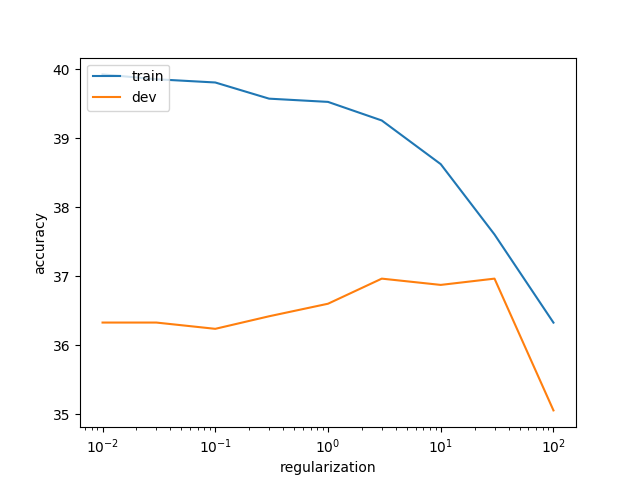
\includegraphics{assignment1/q4_reg_v_acc.png}

We see that training accuracy falls as the regularization value goes up, which makes sense - a lower regularization value gives the model ``more freedom" to fit the training data more closely. We also see that dev accuracy is lower for low regularization values, indicating overfitting, and that dev accuracy drops sharply after a regularization value of 30, indicating underfitting.

(f)

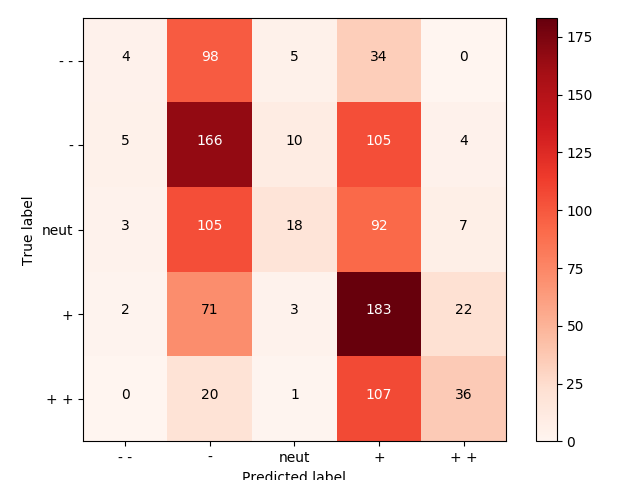
\includegraphics{assignment1/q4_dev_conf.png}

We see that the model appears to have a strong bias for predicting labels 1 and 3 (in particular, the model predicts far more items in those categories than there are in the actual dataset). Given this, however, the model appears to do reasonably well and seems to misclassify few true 4's as 1's and few true 0's as 3's.

(g)
\begin{itemize}
\item ``and if you 're not nearly moved to tears by a couple of scenes , you 've got ice water in your veins ." (Predicted: 1, Actual: 3)
\begin{itemize}
\item The classifier probably learned a negative sentiment on the word ``tears" (and maybe also ``ice" and ``water"), causing it to misclassify this sentence due to being unable to learn on the phrase ``moved to tears" and not being able to identify the contrasting nature of this sentence (it's making a positive statement by juxtaposing two negatives).
\end{itemize}
\item ``there 's enough melodrama in this magnolia primavera to make pta proud yet director muccino 's characters are less worthy of puccini than they are of daytime television ." (Predicted: 4, Actual: 2)
\begin{itemize}
\item There appears to be lots of positive words here (``proud", ``puccini", ``worthy"), but the qualification of ``worthy" with ``less" was probably not picked up on by the classifier, and perhaps the negative sentiment of ``television" was not enough to overcome those positive words.
\end{itemize}
\item ``with the exception of some fleetingly amusing improvisations by cedric the entertainer as perry 's boss , there is n't a redeeming moment here ." (Predicted: 1, Actual: 0)
\begin{itemize}
\item The model probably detected a positive word (amusing) but, being a bag-of-words model, failed to see that ``amusing" was qualified by ``fleetingly", lessening its contribution to the overall meaning of the sentence.
\end{itemize}
\end{itemize}
\end{document}
